\documentclass[10pt,openany]{book}
\usepackage[utf8]{inputenc}
\DeclareUnicodeCharacter{2212}{\ensuremath{-}}
\DeclareUnicodeCharacter{2192}{\ensuremath{\to}}
\DeclareUnicodeCharacter{03B1}{\ensuremath{\alpha}}
\usepackage[T1]{fontenc}
\usepackage{lmodern}
\AtBeginDocument{\normalfont\DeclareFontShape{T1}{lmr}{bx}{sc}{<->ssub*lmr/m/sc}{}}
\usepackage[spanish,es-nodecimaldot]{babel}
\spanishplainpercent
\AtBeginDocument{\spanishdeactivate{"~<>}}
\usepackage[a4paper,margin=2.5cm,headheight=14pt]{geometry}
\usepackage{amsmath,amssymb,mathtools,booktabs,array,longtable,graphicx,xcolor,tikz,enumitem,microtype,titlesec,fancyhdr}
\usepackage[breakable,skins]{tcolorbox}
\usepackage[labelfont=bf]{caption}
\usepackage[hyphens]{url}
\usepackage[hidelinks,unicode,hypertexnames=false]{hyperref}
\definecolor{studiumInk}{RGB}{20,44,64}
\definecolor{studiumBlue}{RGB}{24,74,130}
\definecolor{studiumCyan}{RGB}{0,184,205}
\definecolor{studiumLight}{RGB}{232,240,250}
\definecolor{studiumWorkedBack}{RGB}{255,244,230}
\definecolor{studiumWorkedFrame}{RGB}{138,78,12}
\definecolor{studiumCheckBack}{RGB}{243,236,248}
\definecolor{studiumCheckFrame}{RGB}{96,48,130}
\titleformat{\chapter}[display]{\normalfont\filright}{\large\mdseries\scshape\chaptertitlename\ \thechapter}{1ex}{\normalfont\huge\bfseries}
\titlespacing*{\chapter}{0pt}{2.5ex plus 1ex minus .2ex}{2.3ex}
\titleformat{name=\chapter,numberless}[display]{\normalfont\filright}{}{0pt}{\normalfont\huge\bfseries}
\titleformat{\section}{\Large\bfseries}{\thesection}{.8em}{}
\titleformat{\subsection}{\large\bfseries}{\thesubsection}{.7em}{}
\makeatletter
\renewcommand*\l@section{\@dottedtocline{1}{1.5em}{3.5em}}
\makeatother
\setcounter{secnumdepth}{2}\setcounter{tocdepth}{1}
\setlength{\parindent}{1.5em}\setlength{\parskip}{3pt plus .5pt}
\setlength{\emergencystretch}{1.5em}\raggedbottom
\setlist{itemsep=2pt,topsep=4pt,leftmargin=*}
\setlist[description]{style=nextline,leftmargin=0pt,labelwidth=0pt,labelindent=0pt}
\allowdisplaybreaks[2]
\graphicspath{{../figures/}}
\newcommand{\Raire}{287.05287}
\newcommand{\gzero}{9.80665}
\tcbset{studiumcommon/.style={breakable,boxrule=.65pt,arc=.7pt,left=1.7mm,right=1.7mm,top=1.3mm,bottom=1.3mm,before skip=10pt,after skip=10pt,fonttitle=\bfseries}}
\newtcolorbox{studiumworked}[1]{studiumcommon,colback=studiumWorkedBack,colframe=studiumWorkedFrame,colbacktitle=studiumWorkedFrame,coltitle=white,title={#1}}
\newcommand{\objetivos}[1]{\par\noindent\textbf{Objetivos de aprendizaje.} \textit{#1}\par\medskip}
\newcommand{\caja}[2]{\begin{tcolorbox}[studiumcommon,colback=studiumLight,colframe=studiumBlue,colbacktitle=studiumBlue,coltitle=white,title={#1}]#2\end{tcolorbox}}
\newcommand{\resumen}[1]{\begin{tcolorbox}[studiumcommon,colback=studiumCheckBack,colframe=studiumCheckFrame,colbacktitle=studiumCheckFrame,coltitle=white,title=Resumen]#1\end{tcolorbox}}
\newcommand{\figura}[2]{\begin{figure}[tbp]\centering\includegraphics[width=.83\linewidth]{#1.pdf}\caption{#2}\label{fig:#1}\end{figure}\noindent La figura~\ref{fig:#1} ofrece una representación del modelo discutido.}
\pagestyle{fancy}\fancyhf{}
\fancyhead[LE]{\small\thepage\hspace{1.5em}\mdseries\scshape\nouppercase{\leftmark}}
\fancyhead[RO]{\small\mdseries\scshape\nouppercase{\rightmark}\hspace{1.5em}\thepage}
\renewcommand{\headrulewidth}{.4pt}\renewcommand{\footrulewidth}{0pt}
\fancypagestyle{plain}{\fancyhf{}\fancyfoot[C]{\small\thepage}\renewcommand{\headrulewidth}{0pt}}
\newcommand{\portada}[2]{\hypersetup{pageanchor=false}\begin{titlepage}\thispagestyle{empty}
\begin{tikzpicture}[remember picture,overlay,x=1pt,y=-1pt]
\begin{scope}[shift={(current page.north west)}]
\clip (0,0) rectangle (595.276,841.89);
\node[inner sep=0pt] at (297.638,420.945){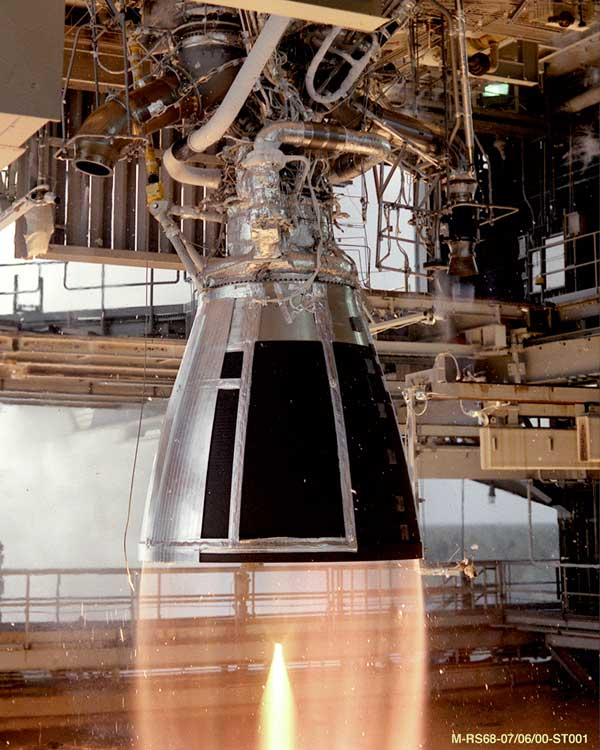
\includegraphics[height=\paperheight]{RS-68_rocket_engine_test.jpg}};
\fill[white,opacity=.91] (0,0) rectangle (595.276,89.5);
\fill[studiumInk,opacity=.96] (0,585.5) rectangle (595.276,841.89);
\node[anchor=west,text=studiumInk,font=\sffamily\bfseries\fontsize{18}{20}\selectfont,inner sep=0pt] at (51.223,38.5){STUDIUM};
\fill[studiumCyan] (51.223,61.5) rectangle (80.8,63.7);
\node[anchor=west,text=studiumInk,font=\sffamily\fontsize{9}{11}\selectfont,inner sep=0pt] at (89.49,65.5){BIBLIOTECA DE INGENIERÍA};
\node[anchor=west,text=studiumCyan,font=\sffamily\bfseries\fontsize{10}{12}\selectfont,inner sep=0pt] at (51.223,608){MANUAL UNIVERSITARIO};
\node[anchor=north west,text=white,text width=493pt,font=\rmfamily\bfseries\fontsize{33}{36}\selectfont,inner sep=0pt] at (51.223,636){#1};
\node[anchor=west,text=white!82!studiumInk,font=\sffamily\fontsize{11}{14}\selectfont,inner sep=0pt] at (51.223,732){#2};
\node[anchor=west,text=white,font=\sffamily\bfseries\fontsize{10}{12}\selectfont,inner sep=0pt] at (51.223,758){GRADO EN INGENIERÍA AEROESPACIAL};
\node[anchor=west,text=white!82!studiumInk,font=\sffamily\fontsize{10}{12}\selectfont,inner sep=0pt] at (51.223,773){Universidad de León};
\draw[white!75!studiumInk,line width=.4pt] (51.223,786) -- (544.05,786);
\node[anchor=west,text=white!82!studiumInk,font=\sffamily\fontsize{10}{12}\selectfont,inner sep=0pt] at (51.223,810){2026};
\node[anchor=east,text=white,font=\sffamily\bfseries\fontsize{10}{12}\selectfont,inner sep=0pt] at (544.05,810){I Edición};
\end{scope}\end{tikzpicture}\null\end{titlepage}\hypersetup{pageanchor=true}}
